\documentclass[a4paper, 10pt]{article}

\usepackage{graphicx}

\title{Architettura degli Elaboratori}

\begin{document}
	\maketitle
	
	\section{Introduzione}
		\textbf{Ci tengo a ricordare che questi sono solo esempi e non rappresentano in alcun modo l'esatto contenuto dell'esame in questione.\\ \\ Ogni esempio contenuto in questo documento e' stato realizzato da Mirco De Marchi.}
		
	\section{Codifica dell'informazione}
		\subsection{Meno Infinito}
			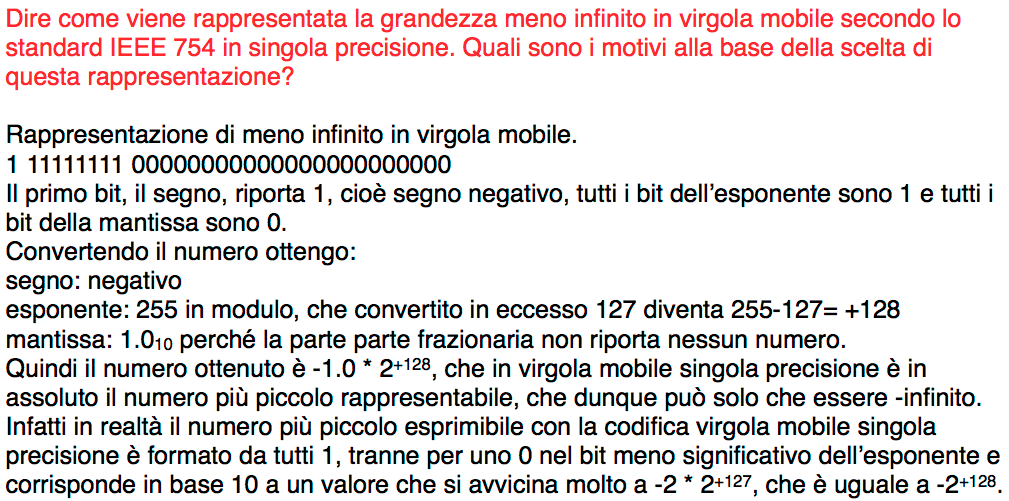
\includegraphics[width=\textwidth]{meno_infinito.png}
			
		\subsection{Somma in complemento a 2}
			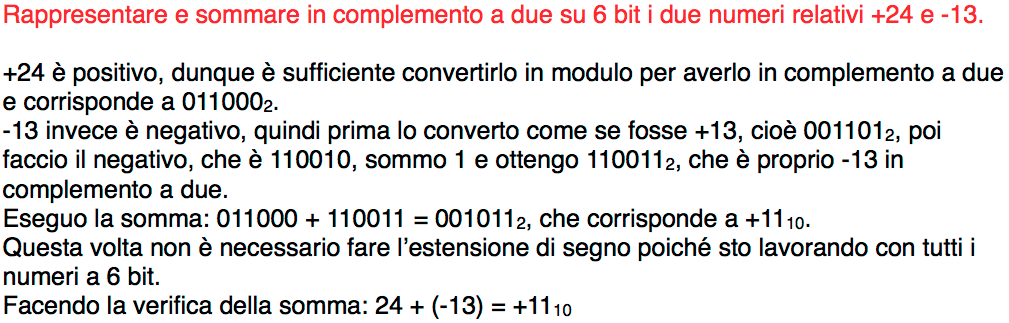
\includegraphics[width=\textwidth]{somma_complemento.png}
			
		\subsection{Cambio da Complemento a 2 a Modulo}
			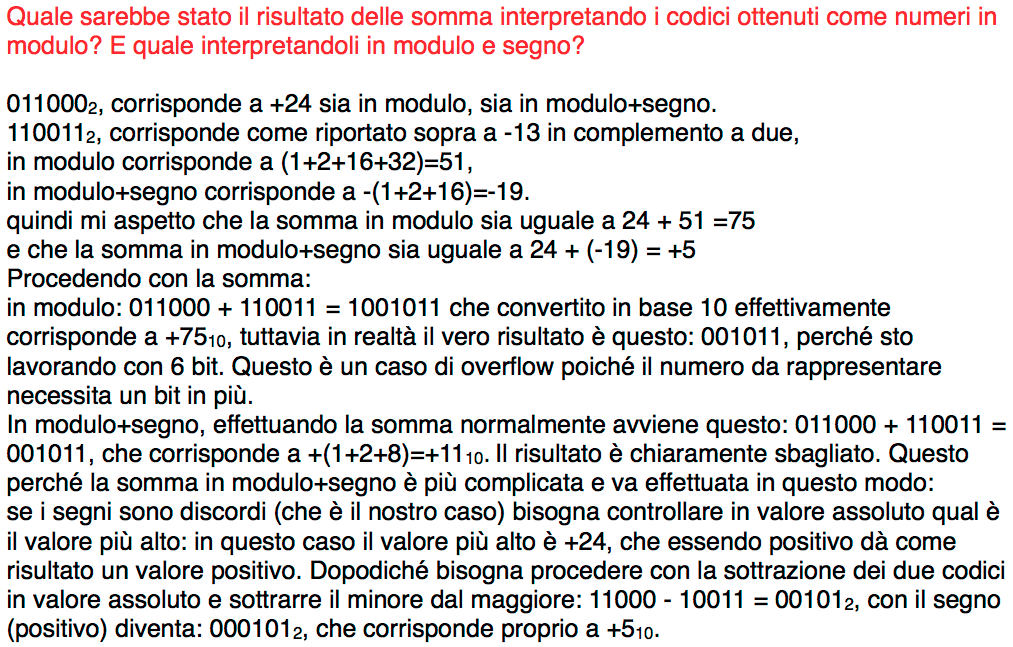
\includegraphics[width=\textwidth]{Cambio_in_modulo.png}
			
	\section{Macchine a Stati Finiti}
		Esempio fornito nel PDF: \textit{FSM.pdf}
		
	\section{Semplificazione Quine-McCluskey}
		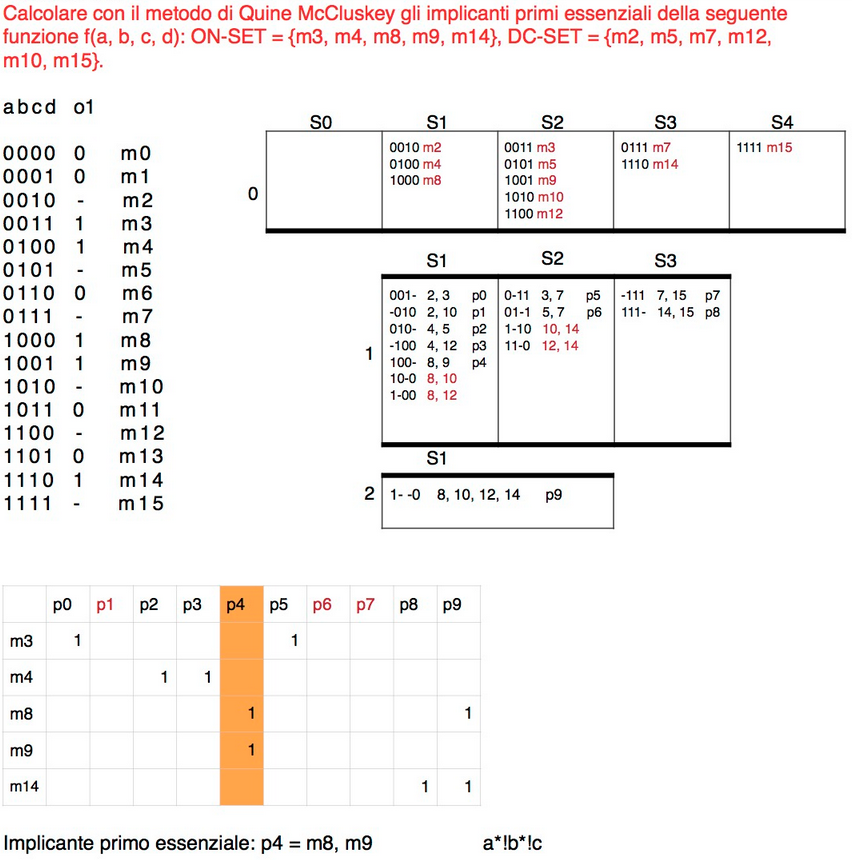
\includegraphics[width=\textwidth]{Semplificazione_QM.png} 
	
		
\end{document}